\chapter{Fluid-structure interaction}
\label{sec:fsi}
We model FSI with the transport velocity formulation scheme, as it is
advantageous as it can solve the tensile instability issue in solid dynamics and
ensure a homogeneous particle distribution in fluids without any additional
artificial stress terms. We model FSI by the CTVF method, where both fluids and
solid phases are modeled using CTVF alone. While the interaction is modeled
using a dummy particle approach \citep{Adami2012}. We additionally consider the
force acting on fluid particles due to the interaction with the structure in the
momentum equation. A similar modification is carried out to the solid particle
momentum equation as well.

\section{Interaction force}\label{subsec:fsi}
Coupling is handled in a straight forward way in SPH. While modelling the fluid
phase and treating the fluid-structure interactions, the solid particles are
assumed to be boundary particles. From the boundary handling given in Adami
\citep{Adami2012}, we compute the pressure of the boundary particles from
the extrapolated equation as,
\begin{equation}
  \label{eq:fsi:pressure-bc}
  p_s = \frac{\Sigma_f p_f W_{sf} + (\ten{g} - \ten{a}_{\ten{s}}) \cdot \Sigma_f
    \rho_f \ten{r}_{sf} W_{sf}}{\Sigma_f W_{sf}}.
\end{equation}
Here, $\ten{a}_s$ is the acceleration of the structure particles. The subscript
$f$ denotes the fluid particles and $s$ denotes the solid particles. Using the
extrapolated pressure, the hydrodynamic density of solid particles are
computed. Please note that the pressure we set here only pertain to the
FSI force and does not correspond to the real pressure or density of the
solid particles. By utilizing the previously set hydrodynamic properties on
the structure, the interaction force is computed using,
\begin{equation}
  \ten{F}_{\text{FSI}}^f = -m_f \sum_{s} m_s \bigg(\frac{p_f}{\rho_{f}^2} +
  \frac{p_s}{\rho_{s}^2} + \Pi_{fs} \bigg) \nabla_{f} W(x_{fs}).
\end{equation}


\section{Water impact onto an elastic plate}
\label{sec:water-impact-forefront}
We study the deformation of the elastic plate due to the impact of water from a
dam break. The material properties of the elastic plate with a density of $2500$
kgm\textsuperscript{-3}, Young's modulus of $10^6$ Pa, and a Poisson ratio of
$0$. The material properties of the fluid are a density of 1000
kgm\textsuperscript{-3}, with no dynamic viscosity. In
\cref{fig:dam-breaking-onto-plate-snapshot}, we show the schematic of the elastic
dam break, and the deformed structure with fluid rise at a time instant.
\Cref{fig:water-impact-plate-deflection-quantitative} compares displacement of
the tip of the structure simulated with the current solver to other numerical
implementations.
\begin{figure}[!htpb]
    \centering
  \begin{subfigure}{0.48\textwidth}
    \centering
    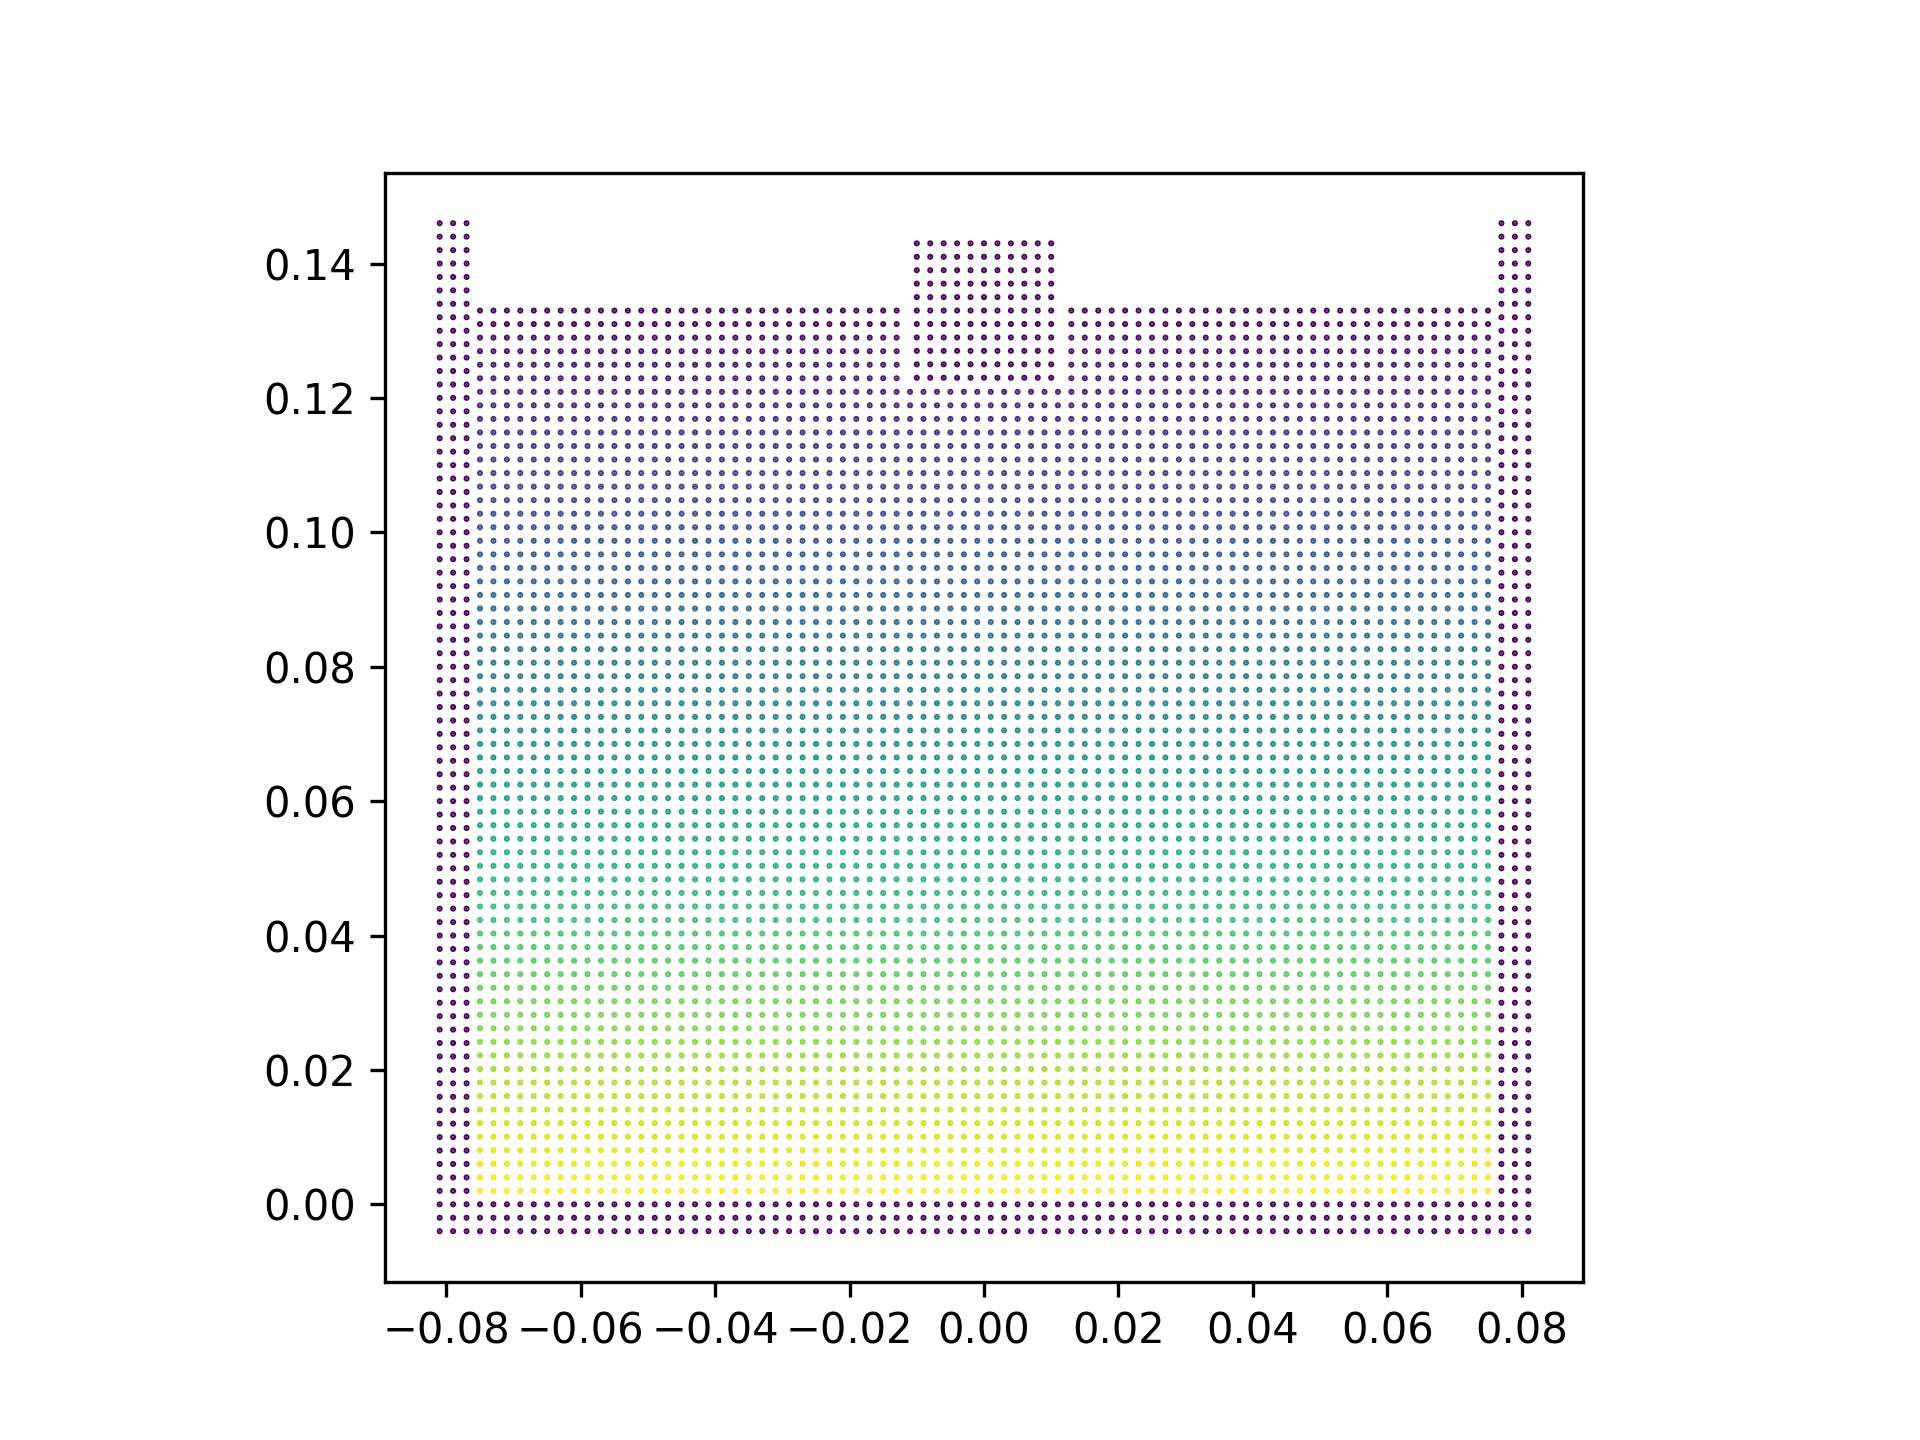
\includegraphics[scale=0.3]{images/fsi/images/sun_2019_dam_breaking_flow_impacting_an_elastic_plate/schematic}
    \caption{}
  \end{subfigure}
  \begin{subfigure}{0.48\textwidth}
    \centering
        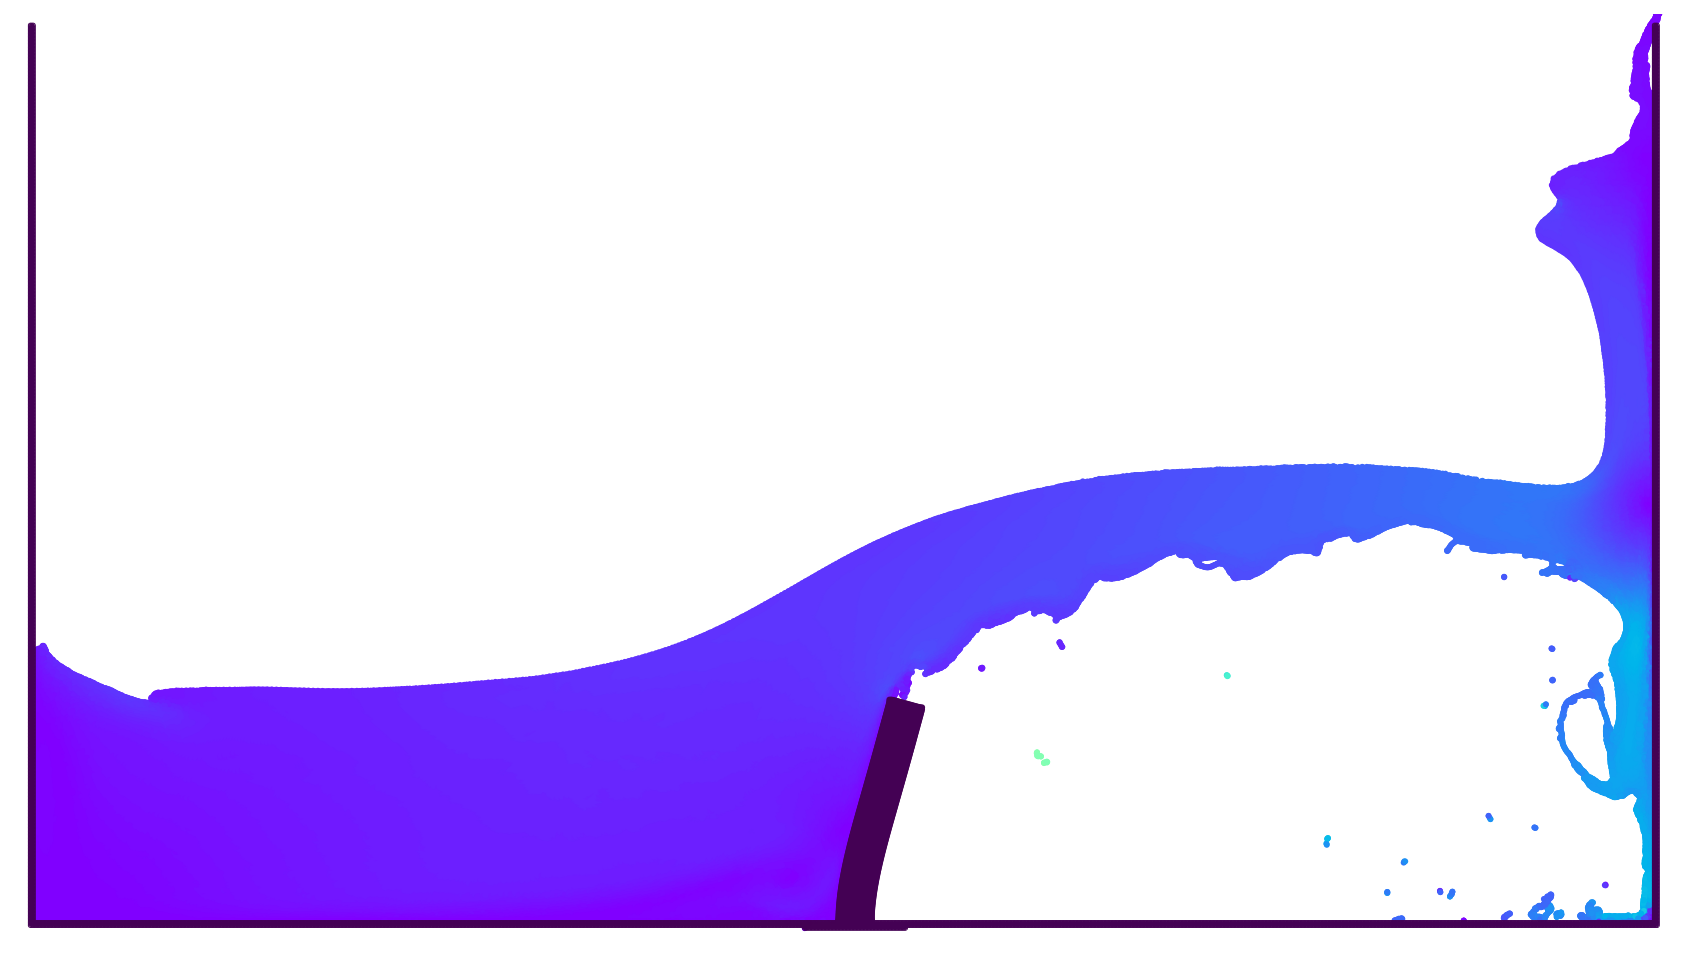
\includegraphics[scale=0.4]{figures/fsi/figures/sun_2019_dam_breaking_flow_impacting_an_elastic_plate/snap_t_2.png}
        \caption{}
  \end{subfigure}
    \caption
    { (a) Schematic of dam break flow over an elastic obstacle. (b) Snapshot of
      the deformed structure obstructing the fluid. }
    \label{fig:dam-breaking-onto-plate-snapshot}
\end{figure}
\begin{figure}[!htpb]
  \centering
  \includegraphics[scale=0.45]{figures/fsi/figures/sun_2019_dam_breaking_flow_impacting_an_elastic_plate/x_amplitude}
  \caption{Time histories of horizontal displacement of the free end of the
    elastic structure compared against the numerical results of
    \citep{sun2019fully,bogaers2016evaluation}- Water impact onto an elastic
    plate.}
\label{fig:water-impact-plate-deflection-quantitative}
\end{figure}
